\documentclass[twoside]{scrartcl}
\usepackage{freitag}
\usepackage{tikz}
\usepackage{xfp}
\usetikzlibrary{math}
\usetikzlibrary{positioning}

\tikzmath{\bandheight = 16;}

\newcommand{\assignment}[3]{\draw [#1] (0em, \bandtranslate{#2}) rectangle (0.5em, \bandtranslate{#3});}
\newcommand{\bandlower}{}
\newcommand{\bandtranslate}[1]{\fpeval{\bandheight cm - (#1 - \bandlower) * \bandscale}}
\newcommand{\bw}[3]{\draw [#1] (0.5em, \bandtranslate{#2}) rectangle (1.25em, \bandtranslate{#3});}
\newcommand{\freq}[2][mid]{\draw (2.75em, \bandtranslate{#2}) node [#1] {#2};}
\newcommand{\legend}[3][]{\node (#2) [#2, legend, label={[label distance=1em]0:#3}, #1] {};}
\newcommand{\mode}[3]{\draw [#1] (1.25em, \bandtranslate{#2}) rectangle (2.75em, \bandtranslate{#3});}

\newenvironment{band}[2]{\noindent
  \begin{minipage}[t]{7em}
	\vspace{0pt}
  \begin{tikzpicture}
  \renewcommand{\bandlower}{#1}
	\tikzmath{
		\bandspan = \fpeval{#2 - #1};
		\bandscale = \bandheight / \bandspan;
	}
	\freq[start]{#1}
	\freq[end]{#2}
}
{\end{tikzpicture}\end{minipage}}

\newenvironment{bandnotes}{\begin{minipage}[t]{\dimexpr\linewidth-7.3em\relax}
	\vspace{0.38em}
	\begin{description}
}{\end{description}\end{minipage}}

% Modes
\tikzstyle{cw} = [fill=red, line width=1pt, draw=white]
\tikzstyle{data} = [fill=yellow, line width=1pt, draw=white]
\tikzstyle{ssb} = [fill=green, line width=1pt, draw=white]
\tikzstyle{voice} = [fill=blue, line width=1pt, draw=white]
\tikzstyle{all} = [fill=cyan, line width=1pt, draw=white]
\tikzstyle{rpt} = [fill=magenta, line width=1pt, draw=white]
\tikzstyle{sat} = [fill=violet, line width=1pt, draw=white]
\tikzstyle{none} = [fill=base03, line width=1pt, draw=white]

% Bandwidth
\tikzstyle{20} = [fill=base03, line width=1pt, draw=white]
\tikzstyle{200} = [fill=base02, line width=1pt, draw=white]
\tikzstyle{500} = [fill=base01, line width=1pt, draw=white]
\tikzstyle{1000} = [fill=base00, line width=1pt, draw=white]
\tikzstyle{2700} = [fill=base0, line width=1pt, draw=white]
\tikzstyle{6000} = [fill=base1, line width=1pt, draw=white]
\tikzstyle{12k} = [fill=base2, line width=1pt, draw=white]
\tikzstyle{20k} = [fill=base3, line width=1pt, draw=white]

% Allocation
\tikzstyle{primary} = [fill=base2, line width=1pt, draw=white]
\tikzstyle{secondary} = [fill=base1, line width=1pt, draw=white]

% Label position
\tikzstyle{start} = [anchor=north west]
\tikzstyle{mid} = [anchor=west]
\tikzstyle{end} = [anchor=south west]

\tikzstyle{legend} = [minimum size=1.8em]

\definecolor{base03}{RGB}{0,43,54}
\definecolor{base02}{RGB}{7,54,66}
\definecolor{base01}{RGB}{88,110,117}
\definecolor{base00}{RGB}{101,123,131}
\definecolor{base0}{RGB}{131,148,150}
\definecolor{base1}{RGB}{147,161,161}
\definecolor{base2}{RGB}{238,232,213}
\definecolor{base3}{RGB}{253,246,227}
\definecolor{yellow}{RGB}{181,137,0}
\definecolor{orange}{RGB}{203,75,22}
\definecolor{red}{RGB}{220,50,47}
\definecolor{magenta}{RGB}{211,54,130}
\definecolor{violet}{RGB}{108,113,196}
\definecolor{blue}{RGB}{38,139,210}
\definecolor{cyan}{RGB}{42,161,152}
\definecolor{green}{RGB}{133,153,0}

\begin{document}
\inlaytitlepage{Bandplan}
\addsec{Bandplan Legend}
\noindent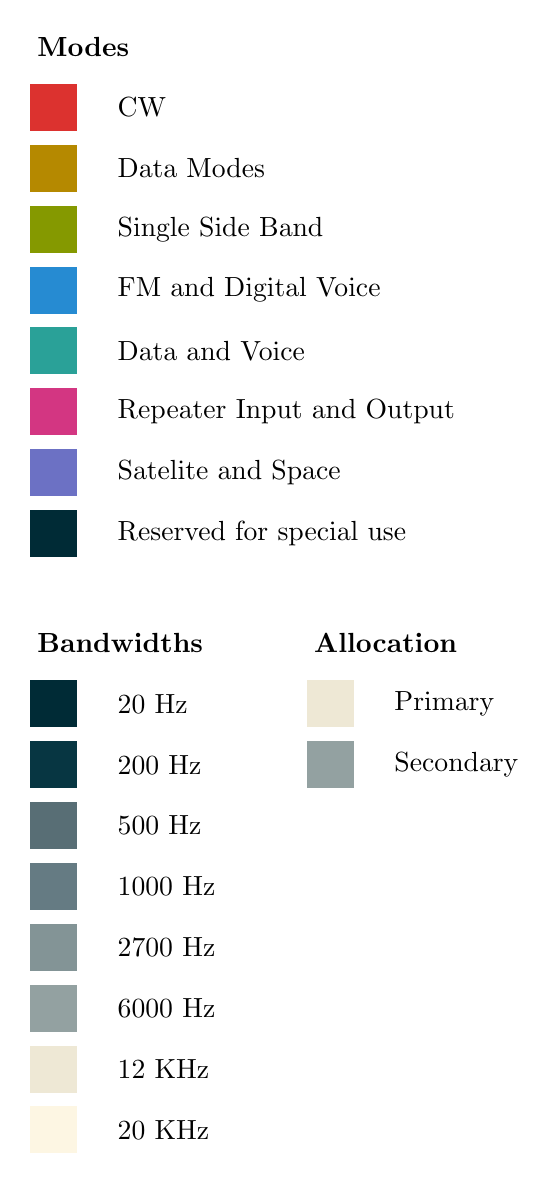
\begin{tikzpicture}[node distance=2.2em]
	\node (modes) {\textbf{Modes}};
	\legend[below=of modes.west, anchor=west]{cw}{CW}
	\legend[below of=cw]{data}{Data Modes}
	\legend[below of=data]{ssb}{Single Side Band}
	\legend[below of=ssb]{voice}{FM and Digital Voice}
	\legend[below of=voice]{all}{Data and Voice}
	\legend[below of=all]{rpt}{Repeater Input and Output}
	\legend[below of=rpt]{sat}{Satelite and Space}
	\legend[below of=sat]{none}{Reserved for special use}

	\node[below=3em of none.south west, anchor=west] (bw) {\textbf{Bandwidths}};
	\legend[below=of bw.west, anchor=west]{20}{20 Hz}
	\legend[below of=20]{200}{200 Hz}
	\legend[below of=200]{500}{500 Hz}
	\legend[below of=500]{1000}{1000 Hz}
	\legend[below of=1000]{2700}{2700 Hz}
	\legend[below of=2700]{6000}{6000 Hz}
	\legend[below of=6000]{12k}{12 KHz}
	\legend[below of=12k]{20k}{20 KHz}

	\node[right=10em of bw.west, anchor=west] (alloc) {\textbf{Allocation}};
	\legend[below=of alloc.west, anchor=west]{primary}{Primary}
	\legend[below of=primary]{secondary}{Secondary}
\end{tikzpicture}

\addsec{1.8 MHZ (160 m) / 1000 W (100 W)}
\begin{band}{1810}{2000}
	\assignment{primary}{1810}{1850}
	\assignment{secondary}{1850}{2000}

	\bw{200}{1810}{1838}
	\bw{500}{1838}{1840}
	\bw{2700}{1840}{2000}

	\freq[end]{1838}
	\freq{1840}
	\freq[start]{1843}
	\freq[start]{1850}

	\mode{cw}{1810}{1838}
	\mode{data}{1838}{1843}
	\mode{ssb}{1843}{2000}
\end{band}
\begin{bandnotes}
	\item[Prefered side band] LSB
	\item[CW QRP calling frequency] 1836 kHz
\end{bandnotes}

\addsec{3.5 MHz (80 m) / 1000 W (100 W)}
\begin{band}{3500}{3800}
	\assignment{secondary}{3500}{3800}

	\bw{200}{3500}{3580}
	\bw{500}{3580}{3600}
	\bw{2700}{3600}{3800}

	\freq{3570}
	\freq{3580}
	\freq{3600}
	\freq{3620}

	\mode{cw}{3500}{3570}
	\mode{data}{3570}{3620}
	\mode{ssb}{3620}{3800}
\end{band}
\begin{bandnotes}
	\item[Prefered side band] LSB
	\item[Emergency Frequency] 3760 kHz
	\item[Activity Centers] \mbox{}
	\begin{description}
		\item[CW QRP] 3555 kHz
		\item[CW QRS] 3555 kHz
		\item[Digital Voice] 3630 kHz
		\item[Image] 3735 kHz
		\item[SSB QRP] 3690 kHz
	\end{description}
\end{bandnotes}

\addsec{5 MHz (60 m) / 15 W EIRP}
\begin{band}{5351.5}{5366.5}
	\assignment{secondary}{5351.5}{5366.5}

	\bw{200}{5351.5}{5354.0}
	\bw{2700}{5354.0}{5366.0}
	\bw{20}{5366.0}{5366.5}

	\freq{5354.0}
	\freq[end]{5366.0}

	\mode{cw}{5351.5}{5354}
	\mode{all}{5354}{5366}
	\mode{data}{5366}{5366.5}
\end{band}
\begin{bandnotes}
	\item[Prefered side band] USB
\end{bandnotes}

\addsec{7 MHz (40 m) / 1000 W}
\begin{band}{7000}{7200}
	\assignment{primary}{7000}{7200}

	\bw{200}{7000}{7040}
	\bw{500}{7040}{7050}
	\bw{2700}{7050}{7200}

	\freq{7040}
	\freq{7050}
	\freq{7060}

	\mode{cw}{7000}{7040}
	\mode{data}{7040}{7060}
	\mode{ssb}{7060}{7200}
\end{band}
\begin{bandnotes}
	\item[Prefered side band] LSB
	\item[Emergency Frequency] 7110 kHz
	\item[Activity Centers] \mbox{}
	\begin{description}
		\item[CW QRP] 7030 kHz
		\item[Digital Voice] 7070 kHz
		\item[Image] 7165 kHz
		\item[SSB QRP] 7090 kHz
	\end{description}
\end{bandnotes}

\addsec{10 MHz (30 m) / 1000 W}
\begin{band}{10100}{10150}
	\assignment{secondary}{10100}{10150}

	\bw{200}{10100}{10130}
	\bw{500}{10130}{10150}

	\freq{10130}

	\mode{cw}{10100}{10130}
	\mode{data}{10130}{10150}
\end{band}
\begin{bandnotes}
	\item[Emergency] 10.138 MHz USB
	\item[Activity Centers] \mbox{}
	\begin{description}
		\item[CW QRP] 10116 kHz
	\end{description}
\end{bandnotes}

\addsec{14 MHz (20 m) / 1000 W}
\begin{band}{14000}{14350}
	\assignment{primary}{14000}{14350}

	\bw{200}{14000}{14070}
	\bw{500}{14070}{14099}
	\bw{2700}{14101}{14350}

	\freq{14070}
	\freq[end]{14099}
	\freq[start]{14101}

	\mode{cw}{14000}{14070}
	\mode{data}{14070}{14099}
	\mode{none}{14099}{14101}
	\mode{ssb}{14101}{14350}
\end{band}
\begin{bandnotes}
	\item[Prefered side band] LSB
	\item[Emergency] 14300 kHz
	\item[Activity Centers] \mbox{}
	\begin{description}
		\item[CW QRS] 14055 kHz
		\item[CW QRP] 14600 kHz
		\item[Digital Voice] 14130 kHz
		\item[Image] 14230 kHz
		\item[SSB QRP] 14285 kHz
	\end{description}
	\item[Priority for DX-peditions] \mbox{} \\ 14195 ±5 kHz
\end{bandnotes}

\addsec{18 MHz (17 m) / 1000 W}
\begin{band}{18068}{18168}
	\assignment{primary}{18068}{18168}

	\bw{200}{18068}{18095}
	\bw{500}{18095}{18109}
	\bw{2700}{18111}{18168}

	\freq{18095}
	\freq[end]{18109}
	\freq[start]{18111}
	\freq{18120}

	\mode{cw}{18068}{18095}
	\mode{data}{18095}{18109}
	\mode{none}{18109}{18111}
	\mode{data}{18111}{18120}
	\mode{ssb}{18120}{18168}
\end{band}
\begin{bandnotes}
	\item[Prefered side band] USB
	\item[Emergency] 18.160 kHz
	\item[Activity Centers] \mbox{}
	\begin{description}
		\item[CW QRP] 18086 kHz
		\item[Digital Voice] 18150 kHz
		\item[SSB QRP] 18130 kHz
	\end{description}
\end{bandnotes}

\addsec{21 MHz (15 m) / 1000 W (100 W)}
\begin{band}{21000}{21450}
	\assignment{primary}{21000}{21450}

	\bw{200}{21000}{21070}
	\bw{500}{21070}{21110}
	\bw{2700}{21110}{21120}
	\bw{500}{21120}{21149}
	\bw{2700}{21151}{21450}

	\freq{21070}
	\freq{21110}
	\freq{21120}
	\freq[end]{21149}
	\freq[start]{21151}

	\mode{cw}{21000}{21070}
	\mode{data}{21070}{21149}
	\mode{none}{21149}{21151}
	\mode{ssb}{21151}{21450}
\end{band}
\begin{bandnotes}
	\item[Prefered side band] USB
	\item[Emergency] 21360 kHz
	\item[Activity Centers] \mbox{}
	\begin{description}
		\item[CW QRP] 21060 kHz
		\item[CW QRS] 21055 kHz
		\item[Digital Voice] 21180 kHz
		\item[Image] 21340 kHz
		\item[SSB QRP] 21285 kHz
	\end{description}
\end{bandnotes}

\addsec{24 MHz (12 m) / 1000 W}
\begin{band}{24890}{24990}
	\assignment{primary}{24890}{24990}

	\bw{200}{24890}{24915}
	\bw{500}{24915}{24929}
	\bw{2700}{24931}{24990}

	\freq{24915}
	\freq{24929}
	\freq{24931}

	\mode{cw}{24890}{24915}
	\mode{data}{24915}{24929}
	\mode{none}{24929}{24931}
	\mode{ssb}{24931}{24990}
\end{band}
\begin{bandnotes}
	\item[Prefered side band] USB
	\item[Activity Centers] \mbox{}
	\begin{description}
		\item[CW QRP] 24906 kHz
		\item[Digital Voice] 24960 kHz
		\item[SSB QRP] 24950 kHz
	\end{description}
\end{bandnotes}
\end{document}
